\documentclass{ximera}

\title{Ximera Demo}
\author{Andrew}

\begin{document}

\begin{abstract}
    Ximera Demonstration
\end{abstract}


\maketitle

\section{Pythagorean Theorem} The Pythagorean Theorem states that in a right-angle triangle the length of the longest side, the hypotenuse, squared is equal to the sum of one leg squared plus the other leg squared.

\[
{a^2 + b^2 = c^2}
\]

\section{Example} Given the leg $a = 3$ and the hypotenuse $c = 5$, find $b$.

\begin{center}
\begin{tikzpicture}
  \draw (0,0) -- (4,0) -- (4,6) -- cycle; 
  \draw (3.8,0) -- (3.8,0.2) -- (4,0.2); %
   \node[below ] at (2,0) {$a = 3$};
  \node[below] at (4.5,3) {$b$};
  \node[right] at (1,3) {$c = 5$};
\end{tikzpicture}
    
\end{center}

To compute this plug in numbers into the Pythagorean Theorem and solve for $b$:

\[
    a^2 + b^2 = c^2 \rightarrow{3^2 + b^2 = 5^2}
\]
\[
    9 + b^2 = 25 \rightarrow{b^2 = 16};
 \]
\[
    \sqrt{ b } = \sqrt{ 16 }\rightarrow{b = 4};
\]

\section{You Try} Given the legs $b=8$ and $a=5$ find $c$ (the hypotenuse of the right triangle)

\begin{center}
\begin{tikzpicture}
  \draw {(0,0) -- (4,0) -- (4,6) -- cycle};
  \draw (3.8,0) -- (3.8,0.2) -- (4,0.2);
   \node[below ] at (2,0) {$a = 5$};
  \node[below] at (4.5,3) {$b = 8$};
  \node[right] at (1,3) {$c$};
\end{tikzpicture}
\end{center}
\section{The Distance Formula}
The distance formula can be derived from the Pythagorean Theorem. The point $A(x_1,y_1)$ and the point $B(x_2,y_2)$ form a right triangle with the axes. The legs represent the change in the values of $x$ and $y$ and the hypotenuse is the $D$=distance between the two points.
\[
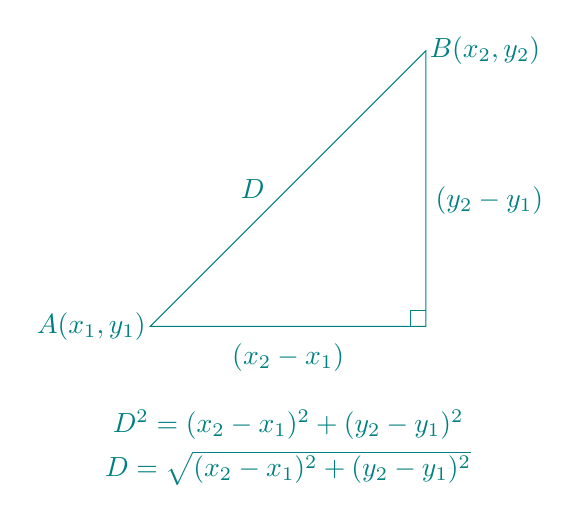
\begin{tikzpicture}
\draw[teal] (0,0) -- (3.5, 0) -- (3.5, 3.5) -- cycle;
\draw[thin, teal]  (3.3, 0) -- (3.3, 0.2)-- (3.5, 0.2);
%\node[right, teal] at (0.2,0.2) {$\theta$}; 
\node[teal] at (-0.75,0) {$A(x_1,y_1)$}; %point a
\node[teal] at (4.25,3.5) {$B(x_2,y_2)$} ; %point b
\node[below, teal] at (1.75,-0.1) {$(x_2-x_1)$}; %adjacent
\node[right, teal] at (3.5,1.6) {$(y_2-y_1)$}; %opposite
\node[teal] at (1.75, -1.25) {$D^2 = (x_2-x_1)^2 + (y_2-y_1)^2$};
\node[teal] at (1.75, -1.8) {$D = \sqrt{(x_2-x_1)^2 + (y_2-y_1)^2}$};%hypotenuse
 
%\node[right] at (4.1,2) {$\tan(\theta)$};
\node[above, teal] at (1.3,1.5) {$D$}; %hypotenuse
\end{tikzpicture}
\]

\section{Example} 
Using the distance formula, find the distance between point $(3,-5)$ and $(-6,7)$

Step 1: Plug the points into the distance formula. 
\[
D = \sqrt{(-6-3)^2 + (7-(-5))^2} 
\]
Step 2: Simplify and find distance
\[
D = \sqrt{(-9)^2+(12)^2}
\]
\[
D = \sqrt{81+144}
\]
\[
D = \sqrt{225} \rightarrow D= 15
\]
So, the distance between point $(3,-5)$ and $(-6,7)$ is $15$ units.

\section{You Try}
On a map, the coordinates of the hiker are $(2,5)$ kilometers and they are trying to hike back to their campground at $(7,10)$ kilometers. Assuming the hiker can walk in a straight line and ignoring terrain, use the distance formula to calculate how many kilometers the hiker must walk back to their campsite. Round your answer to the nearest hundredth. (Answer found at the bottom of the page.)

\section{The Equation of a Circle}
A circle is the set of all points in a plane that are the same distance (equidistant) from one point, called the center.
We can find the equation of a circle using the distance point. Seeing that the center is the point $(h,k)$ and the point $(x,y)$ is on the circle, we can find the distance of the radius and the equation of a circle. 
\[
r = \sqrt{(x-h)^2 + (y-k)^2} 
\]
Square both sides to find the equation of a circle.
\[
r^2 =(x-h)^2 + (y-k)^2 
\]
\newpage
\section{Example}
If the center of a circle is $(2,4)$ and the radius is $4$, write the equation of the circle.

Step 1: Plug in information into the equation of a circle
\[
(x-2)^2+(y-4)^2=16
\]
We can also graph this, plot the center and draw the radius to create a circle
\[
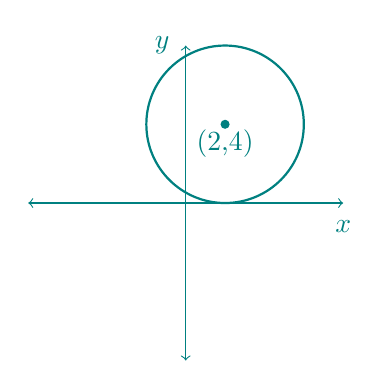
\begin{tikzpicture}
    \draw[teal,<->] (-2,0) -- (2,0) ; %axis
    \draw[teal,<->] (0,-2) -- (0,2) ;
    \draw[teal,thick] (.5,1) circle (1);
    \filldraw[teal] (.5,1) circle (.05);
    \node[teal] at (.5, .75) {(2,4)};
    \node[teal] at (2,-.3) {$x$};
    \node[teal] at (-.3,2) {$y$};
\end{tikzpicture}
\]

\section{You Try}
Find the equation of a circle given the center $(-1,3)$ and the point {(2,-3)} which is a point on the circle. (Hint: find the radius by using the distance formula to calculate the distance between the center and given point) %Nice example!

Answer key : 7.07 kilometers , $(x+1)^2 + (y-3)^2 = 45$ 
\section{Similar Right Triangles}
In a right triangle, if two triangles have the same acute angle, then the ratio of any two sides is constant. This happens because all right triangles with the same acute angle are similar, which means that the ratio of any two corresponding sides is the same. That is why this constant depends on angle and not side length. 

\[
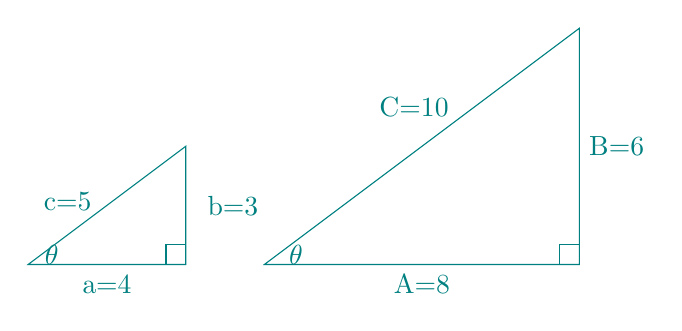
\begin{tikzpicture}
\draw[teal] (-2.5,0) -- (-.5,0) -- (-.5,1.5) -- cycle;
\node[teal] at (-1.5,-.25) {a=4} ;
\node[teal] at (.1,.75) {b=3} ;
\node[teal] at (-2, .8) {c=5};
\node[teal] at (-2.2, 0.125) {$\theta$} ;
\draw[teal,thin] (-.75,0) -- (-.75,.25) -- (-.5,.25) -- (-.5,0) -- cycle;

\draw[teal] (.5,0) -- (4.5,0) -- (4.5,3) -- cycle;
\node[teal,below] at (2.5,0) {A=8} ;
\node[teal,right] at (4.5,1.5) {B=6} ;
\node[teal,above] at (2.4,1.75) {C=10};
\node[teal] at (.9,0.125) {$\theta$};
\draw[teal,thin] (4.25,0) -- (4.25,.25) -- (4.5,.25) -- (4.5,0) -- cycle;

\end{tikzpicture}
\]

If we find the rations of the corresponding sides, we will find that
\[
\frac{a}{b} = \frac{A}{B} \rightarrow \frac{4}{3} = \frac{8}{6}
\]
This works for all ratios. All ratios are constant because they are similar triangles, which is dictated by the angle.

\section{Trigonometric Angles}
When given a right triangle, we can find the functions $sin$, $cos$, and $tan$ of any given acute angle.

\[
sin(\theta) = \frac{opposite}{hypotenuse}
cos(\theta) = \frac{adjacent}{hypotenuse}
tan(\theta) = \frac{oppostie}{adjecent}
\]

\[
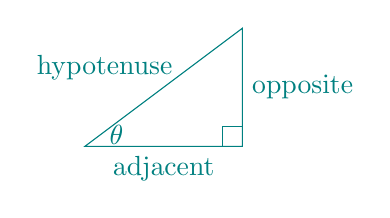
\begin{tikzpicture}
    \draw[teal] (0,0) -- (2,0) -- (2,1.5) -- cycle;
    \node[teal] at (.4,.15) {$\theta$};
    \node[teal,below] at (1,0) {adjacent};
    \node[teal,right] at (2,.75) {opposite};
    \node[teal] at (0.25,1) {hypotenuse};
    \draw[teal,thin] (1.75,0) -- (1.75,.25) -- (2,.25) -- (2,0) -- cycle;
\end{tikzpicture}
\]

\section{Special Right Triangle 1 : $45^\circ-45^\circ-90^\circ$}
A $45^\circ-45^\circ-90^\circ$ right triangle is a special isosceles right triangle. Since the other two angles (besides the $90^\circ$) are equal, the other two side lengths are equal. We can use the Pythagorean Theorem to find the hypotenuse considering the lengths of the legs are 1. The hypotenuse is $\sqrt{2}$.
\[
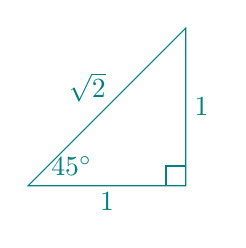
\begin{tikzpicture}
    \draw[teal] (0,0) -- (2,0) -- (2,2) -- cycle;
    \node[teal] at (1,-.2) {1};
    \node[teal] at (2.2,1) {1};
    \node[teal] at (.75,1.25) {$\sqrt{2}$};
    \draw[teal,thin] (1.75,0) -- (1.75,.25) -- (2,.25) -- (2,0) -- cycle;
    \node[teal] at (.55,.25) {$45^\circ$};
\end{tikzpicture}
\]
We can find the values of $sin$, $cos$, and $tan$ of this triangle at the angle $45^\circ$ :
\[
\sin(45^\circ) = \frac{1}{\sqrt{2}}
\cos(45^\circ) = \frac{1}{\sqrt{2}}
\tan(45^\circ) = \frac{1}{1}
\]
Simplify to : 
\[
\sin(45^\circ) = \frac{\sqrt{2}}{2}
\cos(45^\circ) = \frac{\sqrt{2}}{2}
\tan(45^\circ) = 1
\]

\end{document}

